\documentclass[12p,a4paper]{report}
\usepackage[utf8]{inputenc}
\usepackage[T1]{fontenc,url}
\usepackage{multicol}
\usepackage{multirow}
\usepackage{parskip}
\usepackage{lmodern}
\usepackage{microtype}
\usepackage{verbatim}
\usepackage{amsmath, amssymb}
\usepackage{tikz}
\usepackage{physics}
\usepackage{mathtools}
\usepackage{algorithm}
\usepackage{algpseudocode}
\usepackage{listings}
\usepackage{enumerate}
\usepackage{graphicx}
\usepackage{booktabs}
\usepackage{float}
\usepackage{hyperref}
\usepackage{tabularx}
\usepackage{siunitx}
\usepackage{fancyvrb}
\usepackage{blindtext}
\usepackage{tcolorbox}
\usepackage{relsize}
\usepackage[makeroom]{cancel}
\usepackage[margin=1.5cm]{geometry}
\renewcommand{\baselinestretch}{1}
\renewcommand{\exp}{e^}
\renewcommand{\b}{\boldsymbol}
\newcommand{\h}{\hat}
\newcommand{\m}{\mathbb}
\newcommand{\half}{\frac{1}{2}}
\renewcommand{\exp}{e^}
\renewcommand{\bar}{\overline}
\newcommand{\lRightarrow}{\mathlarger{\mathlarger{\Rightarrow}}}
\setlength\parindent{0pt}

%\setlength{\tabcolsep}{6pt} % Default value: 6pt
%\renewcommand{\arraystretch}{1.5} % Default value: 1


\begin{document}


\section*{Random Variables}
A random variable $X$ is a random, quantifiable answer that answers some probabilistic question, like "how many cars will pass here in the next 10 minutes?". The RV will have some underlying theoretical PDF $f(x)$, which will collapse into a single value when observed. Consider it a quantum particle in a superposition.


\begin{align*}
    \underbrace{
        f(x) = N(x;\, \mu=5,\, \sigma=1.5) = \frac{1}{\sqrt{2\pi\sigma^2}}\exp{-(x-\mu)^2/2\sigma^2}
    }_{\text{\textcolor{blue}{Theoretical distribution of RV}} }
    \quad\quad \lRightarrow \quad\quad
    \underbrace{
        X_i = [5.345,\, 7.955,\, 3.895,\, 1.065,\, 4.701,\, 1.696,...]
    }_{\text{\textcolor{red}{Sample of RV}}}
\end{align*}
\begin{figure}[H]
    \centering
    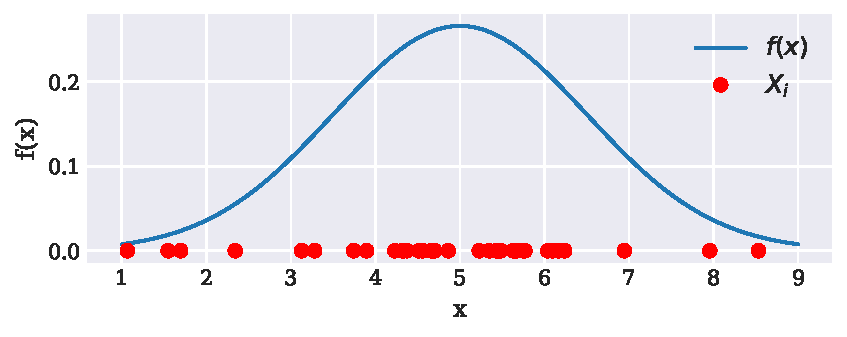
\includegraphics[width=0.7\textwidth]{figs/RV:1.pdf}
    \caption{Random variable $X$, with theoretical PDF $f(x)$, and 35 observations, $X_i$.}
    \label{fig:1}
\end{figure}

\section*{Statistics}
The measured sample $X_i$ will have \underline{statistics} such as mean and standard deviation, mirroring the "actual" values of the theoretical PDF. They will approach the theoretical values as the sample size increases ($N\gg 1$). The most used statistics are the mean $\bar{X}$ and variance $S^2$.

\begin{table}[H]
    \centering
    \begin{tabular}{r  c  c  c  l}\toprule
        \multicolumn{2}{c}{\bf{Properties of PDF - $f(x)$}}  & &  \multicolumn{2}{c}{\bf{Statistics of RV - $X_i$}} \\ \midrule
        Mean  &  $\mu$  & $\leftrightarrow$ &  $\bar{X}$  &  Sample Mean  \\ \midrule
        Variance  &  $V$  & $\leftrightarrow$ &  $S^2$  &  Sample Variance \\ \midrule
        St.Div.  &  $\sigma$  & $\leftrightarrow$ &  $S$  &  Sample St.Div.
    \end{tabular}
    \caption{Properties of the RVs PDF, and the corresponding statistics of a sample of the RV.}
    \label{table:1}
\end{table}

\section*{Distribution of sample statistics}
Since each random sample from the RV will be different, the statistics will differ each time as well, as seen in figure \ref{fig:2}.
\begin{figure}[H]
    \centering
    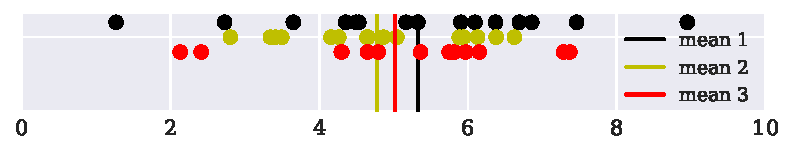
\includegraphics[width=0.6\textwidth]{figs/RV:2.pdf}
    \caption{Three size 15 sample distributions of random variable $X_i$}
    \label{fig:2}
\end{figure}
Imagine picking an infitine amount of such random samples from the RV, each of size $n$. The statistics themselves will now have a distributions, with it's own mean, variance, etc.

\subsection*{Sample mean and Central Limit Theorem}
The \underline{sample mean} of the RV, independently of what sort of distribution the random samples are from, follow
\begin{align}\label{eqn:1}
    E(\bar{X}) = \mu_{\bar{X}} = \mu \quad\quad\quad\quad V(\bar{X}) = \sigma_{\bar{X}}^2 = \sigma^2/n
\end{align}

\subsubsection*{Sample mean of normally distributed RV}
When the RV has a \textbf{normal distribution}, the sample mean $\bar{X}$ is \textbf{itself normally distributed}, with mean and variance as in \ref{eqn:1}:
\[
    Z = \frac{\bar{X} - \mu}{\sigma/\sqrt{n}}
\]
A problem here is that $\sigma$ is often unknown, as it belongs to the theoretical PDF, not the sample.
The \textbf{t distribution} solves the problem. The following random variable has a t-distribution when $\bar{X}$ is the sample mean of a normal RV:
\[
    T = \frac{\bar{X} - \mu}{S/\sqrt{n}}
\]

\subsubsection*{Sample mean of any RV - The Central Limit Theorem (CLT)}
When the RV has \textbf{any distribution}, the sample mean $\bar{X}$ will \textbf{approach a normal distribution} for large $n$. This is called the \underline{central limit theorem}. We can then use both the Z and T distributions as above.


\section*{Point Estimators}
\underline{Estimators} $\hat{\theta}$ are attempts at reconstructing a theoretical parameter (left side of \ref{table:1} - $\mu$, $\sigma$,...) from the sample statistics (right side of \ref{table:1} - $\bar{X}$, $S$,...). The most obvious estimators are simply the mirroring statistics, but there are more advanced ones.
Some definitions:
\begin{itemize}
    \item \textbf{Mean Square Error:} $\text{MSE} = E\qty[(\hat{\theta} - \theta)^2] = V(\hat{\theta}) + E(\hat{\theta}) - \theta = \text{variance of estimator} + \text{bias}^2$
    \item \textbf{Unbiased Estimator:} Estimator which variance is zero $V(\hat{\theta}) = 0$.
    \item \textbf{Minimum Variance Unbiased Estimator:} Estimator with lowest variance, which has no bias $E(\hat{\theta}) = \theta$.
\end{itemize}

\begin{table}[H]
    \centering
    \begin{tabular}{l | c | c }
        \textbf{Property}    &  \textbf{MVUE of norm. dist.}  & Other Estimators \\ \midrule
        Mean $\mu$           & $\bar{X}$       & $\tilde{X}$, $\bar{X}_{tr(10)}$ \\ \midrule
        Variance $\sigma^2$  & $S^2$           & \\ \midrule
        St.Div. $\sigma$     & --              &
    \end{tabular}
    \caption{Most common estimators of common properties}
    \label{table:2}
\end{table}

\subsection*{Bootstrap point estimation}
\subsection*{Moment estimators}
\subsection*{Maximum likelihood estimators}


\newpage
\section*{Confidence Intervals}
We now know what sort of distributions our estimators have. We can then establish some interval around the estimators mean where we are $100(1-\alpha)\%$ sure that the actual value lies.

\begin{tcolorbox}[width=\textwidth,colback={yellow},title={Deriving Confidence Intervals},colbacktitle=green,coltitle=black,fonttitle=\Large]

    \begin{enumerate}
        \item Find some RV which involves only your estimator (and known values), and has a known probability distribution. Ex, for the estimator $\hat{\mu} = \bar{X}$ we can use the RV
        \[ Z = \frac{\bar{X} - \mu}{\sigma/\sqrt{n}} \]
        which has a normal distribution, as long as $\sigma$ is known, or 
        \[ T = \frac{\bar{X} - \mu}{S/\sqrt{n}} \]
        which has a T distribution. if $\sigma$ is not known.

        \item Use the known distributions' percentiles to establish an interval. Ex, for the normal case:
        \[ P\qty(z_{1 - \alpha/2} < \frac{\bar{X} - \mu}{\sigma/\sqrt{n}} < z_{\alpha/2}) = 100(1-\alpha)\% \]

        \item Solve the inequality for the value to be estimated, in this case $\mu$:
        \[ \bar{X} + z_{1-\alpha/2}\cdot \frac{\sigma}{\sqrt{n}} < \mu < \bar{X} + z_{\alpha/2}\cdot \frac{\sigma}{\sqrt{n}} \quad\quad \lRightarrow \quad\quad \mu \in \qty[\bar{X} \pm z_{\alpha/2}\cdot \frac{\sigma}{\sqrt{n}}] \]
    \end{enumerate}

\end{tcolorbox}  

\subsection*{Useful RVs for finding for finding CIs}
\begingroup
    \setlength{\tabcolsep}{6pt} % Default value: 6pt
    \renewcommand{\arraystretch}{1.5} % Default value: 1
    \begin{table}[H]
        \centering
        \begin{tabular}{l | c | c | c }

            \textbf{Distribution}    &  \textbf{Random Variable} & Estimator & Comments \\ \midrule
            Normal Dist. & \scalebox{1.3}{ $Z = \frac{\bar{X} - \mu}{\sigma/\sqrt{n}}$ }       & $\hat{\mu} = \bar{X}$ & Requires that $\sigma$ is known. \\ \midrule
            
            T Dist. & \scalebox{1.3}{ $T = \frac{\bar{X} - \mu}{S/\sqrt{n}}$ }       & $\hat{\mu} = \bar{X}$ & $n-1$ df. Approaches $Z$ as $N \gg 1$. \\ \midrule

            Chi-squared Dist. & \scalebox{1.3}{ $\chi^2 = \frac{(n-1)S^2}{\sigma^2}$ }       & $\hat{\sigma^2} = S^2$ & $n-1$ df. Take sqrt to get CI for $\sigma$. \\ \midrule

        \end{tabular}
        \caption{RV distributions to use in confidence}
        \label{table:3}
    \end{table}
\endgroup


\subsection*{Parametric Bootstrap CI}
\subsection*{Non-parametric Bootstrap CI}

\end{document}

